\section{Grundlagen}
\begin{frame}{}
    \begin{center}
        Grundlagen
     \end{center}
\end{frame}

\begin{frame}{Ein typisches Freifunk Netz}
    \begin{itemize}
        \item Ein Batman-Adv Netz
        \begin{itemize}
            \item[$\rightarrow$] "Wie ein großer dezentraler Switch"
        \end{itemize}
        \item VPN für die Funkinseln
        \begin{itemize}
            \item Multi-Client zu Multi-Client VPN
            \item Layer-II Netz
            \item Kein internes Routing / Forwarding
        \end{itemize}
        \item Mehrere VPN Server / Gateway
        \begin{itemize}
            \item DHCP
            \item DNS Namensauflösung
            \item Gateway zum Internet / ICVPN
        \end{itemize}
        \item Monitoring
        \begin{itemize}
            \item Karte aller Knoten
        \end{itemize}
    \end{itemize}
\end{frame}

\begin{frame}{Ein typisches Freifunk Netz}
    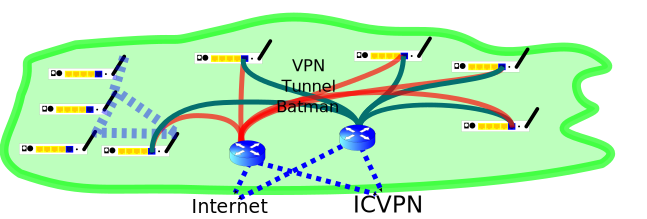
\includegraphics[width=\textwidth]{img/svg/freifunk_konzepte_alt.pdf}
\end{frame}

\begin{frame}{Freifunk Franken Netz}
    \includegraphics[width=\textwidth]{img/svg/freifunk_konzepte.pdf}

    \begin{itemize}
        \item Mehrere Layer-2 Inseln (Hoods)
        \item Verbindung per Layer-3
        \item Dezentrale Gateways
    \end{itemize}
\end{frame}

\begin{frame}{keyXchange V1}
    \begin{itemize}
        \item \glqq{}Automatisches Peering\grqq{}
        \item VPN Endpunkt Vermittlung
        \begin{itemize}
            \item Zentrale Webseite \only<2>{{\color{red}$\rightarrow$ Problem!}}
            \item Knoten meldet sich mit Standort
            \item Geographisch nächste Hood wird zugewiesen (voronoi)
            \item Client bekommt Liste aller Server der Hood
        \end{itemize}
        \item Keine weitere Unterscheidung zu welcher Hood der Knoten gehört
        \begin{itemize}
            \item[$\rightarrow$]<2> {\color{red}Problem!} Funk Verbindung zwischen den Hoods
        \end{itemize}
    \end{itemize}
\end{frame}

\begin{frame}{Gateway}
    \begin{itemize}
        \item VPN Server: In jeder Hood gibt es mehrere davon
        \item Internet: DNS / Gateway
        \begin{itemize}
            \item Adresszuweisung über DHCP (selten: slac)
            \item Anpassung nach Traffic Auslastung: Batman-Adv GW Selection
            \item IPv4 NAT (manchmal übers Ausland) ins Internet
        \end{itemize}
        \item Freifunk: VPN (GRE o. Wireguard) / Routing zu anderen Gateways
        \begin{itemize}
            \item Babel Routing
            \item Routing Metrik ohne Traffic/Bandbreite
            \item Keine Security
        \end{itemize}
    \end{itemize}
\end{frame}
